% Explicar en que consitió el trabajo (brevemente).
	% - Explicar levemente los criterios usados para la paralelización
	% - Por qué es buena idea usar este tipo de procesamiento en filtros de imágenes. (todos los pixeles reciben exactamente el mismo procesamiento y así en una sola ráfaga se peude levantar y procesar muchos).
	% - Explicar la hipótesis (debería ser n veces mas rápido porque zarasa).
	% - Se intentó estudiar si vale la pena o no el esfuerzo adicional de desarrollo y debuggeo.


Para analizar el modelo de procesamiento SIMD se implementaron tres filtros; dos de video\footnote{Los filtros de video implementados son técnicamente filtros de imágenes aplicados a los múltiples cuadros de un video.} y uno de imágenes. Para cada uno de ellos se desarrollaron implementaciones tanto en lenguaje C como en lenguaje ensamblador, utilizando la familia de extensiones SSE (\textbf{S}treaming \textbf{S}IMD \textbf{E}xtensions) de la arquitectura Intel.

Sobre las implementaciones logradas, se estudiaron las diferencias en eficiencia y en costo de desarrollo entre las soluciones en C o en ASM, así como el costo temporal relativo entre las diferentes partes de cada solución. Por ejemplo, se analizó el impacto de los saltos condicionales en una implementación en C o la relación entre tiempo de lectura/escritura, procesamiento y lógica de flujo en un programa en lenguaje ensamblador.

Posteriormente, se compararon las características y la eficiencia de los distintos niveles de optimización provistos por compiladores típicos, así como el beneficio de incorporar variadas estrategias algorítmicas de optimización sobre las implementaciones en lenguaje ensamblador, como la técnica de desenrollado de ciclos en un filtro de video o la técnica de entubado de código en el filtro de imágenes.

Cada una de las experiencias con los tres filtros desarrollados se describen en detalle y por separado en secciones subsiguientes.

\subsection{Modelo de procesamiento SIMD}

	El procesamiento SIMD consiste en realizar una misma operación sobre una gran cantidad de datos de manera simultánea y atómica, logrando lo que se conoce como paralelismo a nivel de datos. Los filtros de imágenes y otros procesos sobre multimedia son particularmente propicios para este tipo de procesamiento ya que habitualmente requieren realizar un mismo tipo de cálculo sobre cientos o miles de puntos, por lo cual la posibilidad de trabajar en bloque provee un claro beneficio en tiempo de ejecución en comparación a un procesamiento en serie.

\begin{figure}[h]
\begin{center}
  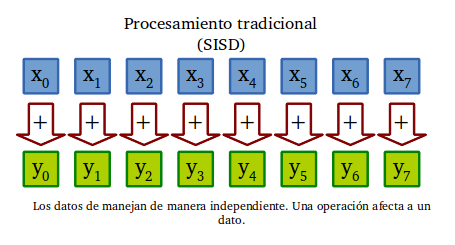
\includegraphics[scale=0.4]{secciones/introduccion/imagenes/SISD.png}
    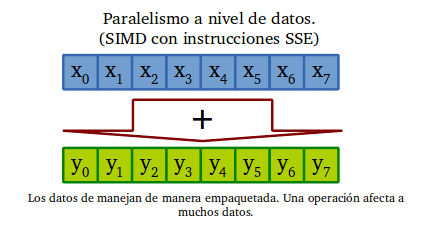
\includegraphics[scale=0.4]{secciones/introduccion/imagenes/SIMD.png}
\end{center}
\caption{Esquemas de procesamiento SISD y SIMD}
\label{fig:SISD-SIMD}
\end{figure}

	Sin embargo para realizar este análisis es imperioso meterse un poco mas adentro.
El comportamiento esperado a priori para estos procesos es una relación inversa entre
el nivel de paralelismo y el tiempo consumido. Es decir, al procesar 4 datos a la vez
uno esperaría obtener que el proceso tarde 4 veces menos tiempo, procesando 8 datos
a la vez 8 veces menos tiempo, etc. Sin embargo esto no siempre ocurre. Durante
este trabajo constantemente se va a intentar explicar que desviaciones se 
produjeron con respecto a este supuesto. Para eso vamos a analizar la arquitectura
intel-64, la velocidad de acceso a memoria, el modo en que se usa la caché,
el medio en el cuál se ejecutan los programas y los algoritmos utilizados entre
otras cosas.

	A lo largo del trabajo se va a ir mostrando como el uso de código de ensamblador
optimizado para el uso de la tecnología SSE produce programas sumamente eficientes. Sin embargo
producir ese código es sumamente trabajoso, mucho mas que usar lenguajes de mas alto nivel como
c o c++. Por ese motivo se intentará hacer otro análisis (tal vez algo menos científico
pero intentando justificar de la manera mas objetiva posible) de cuando vale la pena y cuando no.

Existen también procesos que muestran las limitaciones de este esquema de procesamiento como la lupa con cosenos y la rotación por ejemplo. En general el motivo de estas limitaciones
consiste en que en alguna parte del algorítmo los datos ya no se pueden
tratar mas como un bloque. Por ejemplo en el algoritmo de rotación
uno trae datos consecutivos, los procesa y a la hora de guardarlos
estos no oscupan posiciones consecutivas, por lo tanto a la hora
de grabar los datos no es posible hacerlo utilizando un proceso SIMD.